% IEEE TNSM manuscript. Results produced by the RAS-6G flow-level simulator (October 2026).
\documentclass[letterpaper,journal]{IEEEtran}
\usepackage{amsmath,amssymb,array,booktabs,cite,url}
\usepackage{tikz}
\usetikzlibrary{arrows.meta,calc}
\usepackage{pgfplots}
\usepgfplotslibrary{groupplots}
\pgfplotsset{compat=1.17}
\usepackage{algorithm}
\usepackage{algpseudocode}
\newtheorem{proposition}{Proposition}
\usepackage[hidelinks]{hyperref}
\hyphenation{multi-camera semi-conductor}
\begin{document}
\markboth{IEEE TRANSACTIONS ON NETWORK AND SERVICE MANAGEMENT}%
{Ababneh \MakeLowercase{\textit{et al.}}: Risk-Aware Semantic Utility Optimization for Resilient Multi-Camera Surveillance}
\title{Risk-Aware Semantic Utility Optimization for Resilient Multi-Camera Surveillance in 6G Edge Networks}
\author{Nedal~Ababneh, Khaled~Almi'ani, and Ammar~Kamal~Abasi%
\thanks{N. Ababneh is with the College of Computing and Intelligent Systems, University of Khorfakkan, Sharjah, United Arab Emirates (e-mail: Nedal.Ababneh@ukf.ac.ae).}%
\thanks{K. Almi'ani is with the Faculty of Computer Information Science, Higher Colleges of Technology, Fujairah, United Arab Emirates (e-mail: kalmiani@hct.ac.ae).}%
\thanks{A. K. Abasi is with the Department of Information Systems and Security, College of Computing and Artificial Intelligence, United Arab Emirates University, Al Ain, United Arab Emirates (e-mail: \href{mailto:ammar.abasi@uaeu.ac.ae}{ammar.abasi@uaeu.ac.ae}).}%
\thanks{Corresponding author: Nedal Ababneh (e-mail: \href{mailto:Nedal.Ababneh@ukf.ac.ae}{Nedal.Ababneh@ukf.ac.ae}).}%
}
\maketitle

\begin{abstract}
Mission-critical multi-camera surveillance must preserve timely detection of consequential events when wireless and edge resources degrade. Average detection scores can hide severe misses in critical zones. This paper proposes RAS-6G, a risk-aware semantic utility orchestration framework for 6G-oriented edge networks. The framework jointly selects camera modes, routes and edge servers before disruptions are observed, then adapts admitted streams by frame shedding. A two-stage scenario model bounds the conditional value-at-risk (CVaR) of a severity-weighted, deadline-aware missed-event loss, and a correlation-calibrated surrogate accounts for overlapping views. For online use, a greedy controller applies a Lagrangian CVaR penalty rather than a hard budget. In a flow-level study with 15 topologies and 400 out-of-sample scenarios each, the controller reduced the 95\% CVaR by 26.6\% versus adapted JRRA while using 59\% less bandwidth. An explicit CVaR term cut the risk-neutral variant's tail by 6.2\%, but used more bandwidth; under matched bandwidth and compute budgets the residual CVaR reduction was 3.9\% and not statistically significant. Findings rely on synthetic and literature-inspired detection profiles and require measured multi-view validation.
\end{abstract}
\begin{IEEEkeywords}
6G-oriented edge networks, multi-camera surveillance, semantic utility, resilient service orchestration, CVaR, joint routing and inference.
\end{IEEEkeywords}

\section{Introduction}
\IEEEPARstart{M}{ulti-camera} surveillance has become a core service of public safety, transport and critical infrastructure operators. Real-time video analytics at the network edge has been described as a leading application of edge computing~\cite{ananthanarayanan2017killer}. Moreover, visions of sixth-generation (6G) systems expect the network to support artificial intelligence (AI) services from the core to the end devices~\cite{letaief2019roadmap,saad2020vision}. In such systems, the value of a video stream depends on the task it supports rather than on the number of bits it delivers~\cite{strinati2021sixg,gunduz2023beyond}.

However, multi-camera surveillance over heterogeneous wireless access and edge infrastructure faces coupled constraints. These constraints include transmission capacity, encoder choices, inference throughput and alert deadlines. During congestion, fading or infrastructure failure, reducing every camera's bitrate may preserve throughput. Such a reduction can still fail to deliver timely information from high-consequence locations. Ababneh and Rougier addressed this issue in WiMAX mesh networks by jointly constructing routing trees and assigning rates according to camera utility~\cite{ababneh2012}. Their joint routing and rate allocation (JRRA) formulation used a minimum acceptable bitrate and priority-weighted utility. Today, real-time analytics makes the relevant output an on-time event decision rather than a decodable image.

Recent edge video analytics research coordinates video configurations, bandwidth and shared inference resources~\cite{chen2023survey}. Several systems adapt video configurations to maximize average inference accuracy under bandwidth limits~\cite{jiang2018chameleon,zhang2018awstream,wang2020joint,dai2025biswift}. Notably, average accuracy is a weak indicator for surveillance services that are judged by their worst failures. A high mean detection score can hide a small number of catastrophic misses in a critical zone. Communication research has long recognized that reliability requires attention to the tail of the loss distribution~\cite{bennis2018urllc}. To address such a challenge, risk-aware optimization based on the conditional value-at-risk (CVaR) has emerged as a promising solution~\cite{rockafellar2000,rockafellar2002}. CVaR measures the expected loss in the worst fraction of outcomes and remains tractable in linear programs.

This paper proposes RAS-6G, a risk-aware semantic utility orchestration framework for multi-camera surveillance in 6G-oriented edge networks. Fig.~\ref{fig:architecture} illustrates the architecture of the proposed framework. The framework consists of two main components: a data plane and an orchestration plane. The data plane carries camera streams over wireless and backhaul paths to edge servers that produce zone-level decisions. The orchestration plane selects each camera's mode, route and serving edge under a CVaR-oriented objective (hard constraint offline; penalty online). Link outages, server overload and feed suppression are introduced as evaluation scenarios that remain hidden from the online controller.

\begin{figure*}[!t]
\centering
% All architecture artwork is drawn as vector objects using TikZ.
% No external figure file or additional font/package is required.
\resizebox{\textwidth}{!}{%
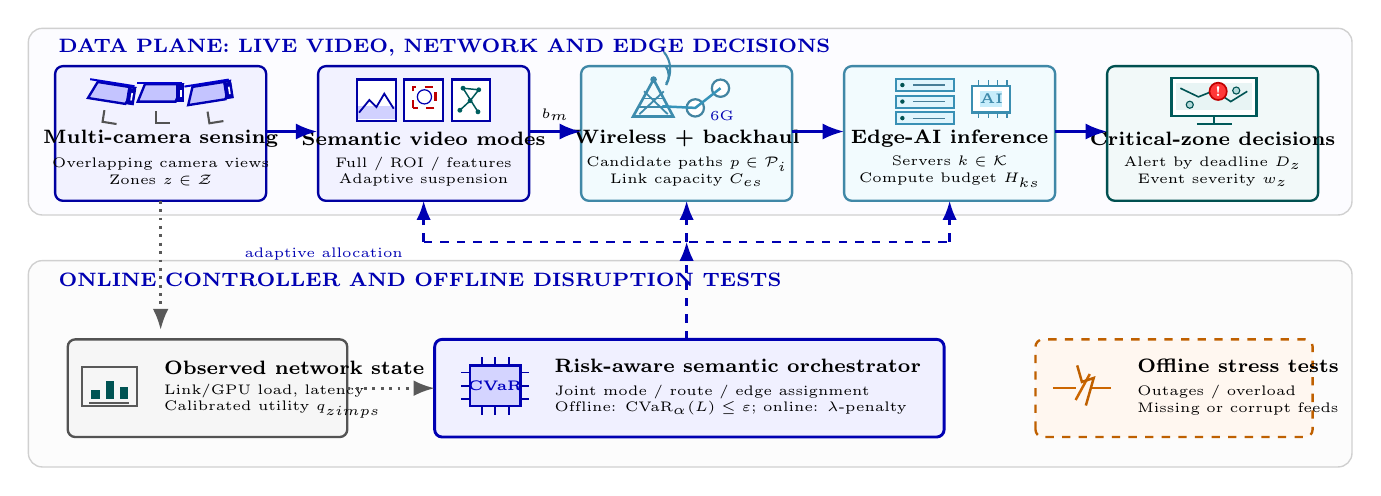
\begin{tikzpicture}[x=1cm,y=1cm,>=Latex,font=\scriptsize,
  frame/.style={draw=blue!55!black,fill=blue!3,rounded corners=3pt,line width=.78pt},
  flow/.style={-Latex,draw=blue!70!black,line width=1.06pt},
  controlarrow/.style={-Latex,draw=blue!70!black,dashed,line width=.86pt},
  measured/.style={-Latex,draw=gray!70!black,dotted,line width=1.03pt}]
% Panel boundaries: data path on top, control and scenario testing below.
\filldraw[rounded corners=5pt,draw=gray!37,fill=blue!1,line width=.5pt]
  (0.10,3.30) rectangle (16.91,5.67);
\filldraw[rounded corners=5pt,draw=gray!37,fill=gray!2,line width=.5pt]
  (0.10,0.10) rectangle (16.91,2.72);
\node[anchor=west,font=\scriptsize\bfseries,text=blue!70!black]
  at (0.36,5.43) {DATA PLANE: LIVE VIDEO, NETWORK AND EDGE DECISIONS};
\node[anchor=west,font=\scriptsize\bfseries,text=blue!70!black]
  at (0.36,2.48) {ONLINE CONTROLLER AND OFFLINE DISRUPTION TESTS};
% Five editable architecture cards with real pictograms.
\foreach \x/\edge in {1.78/blue,5.12/blue,8.46/cyan,11.80/cyan,15.14/teal}{
  \draw[rounded corners=2.8pt,draw=\edge!63!black,fill=\edge!5,line width=.84pt]
    (\x-1.34,3.48) rectangle (\x+1.34,5.19);
}
% CAMERA ILLUSTRATIONS: 3 CCTV cameras with lens hoods and mounting stalks.
\foreach \x/\angle in {1.15/-9,1.78/0,2.41/9}{
  \begin{scope}[shift={(\x,4.78)},rotate=\angle]
    \draw[gray!65!black,line width=.75pt] (-.06,-.16) -- (-.06,-.31) -- (.12,-.31);
    \filldraw[fill=blue!23,draw=blue!70!black,line width=.85pt]
       (-.29,-.04) -- (.19,-.04) -- (.28,.18) -- (-.20,.18) -- cycle;
    \filldraw[fill=blue!70!black,draw=blue!70!black] (.20,-.035) rectangle (.29,.16);
    \draw[white,line width=.6pt] (.255,.015) -- (.255,.11);
    \draw[blue!80!black,line width=.72pt] (-.30,.20) -- (.27,.20);
  \end{scope}
}
% VIDEO/SEMANTIC MODES: full frame, an ROI crop and extracted feature points.
\foreach \x in {4.52,5.12,5.72}{
 \filldraw[fill=white,draw=blue!65!black,line width=.78pt]
  (\x-.245,4.49) rectangle (\x+.245,5.02);
}
\fill[blue!18] (4.29,4.52) rectangle (4.75,4.68);
\draw[blue!65!black,line width=.65pt] (4.30,4.60)--(4.43,4.76)--(4.52,4.67)--(4.62,4.84)--(4.74,4.65);
\draw[red!75!black,dashed,line width=.78pt] (4.98,4.66) rectangle (5.27,4.93);
\draw[blue!70!black,line width=.45pt] (5.13,4.80) circle (.09);
\foreach \xx/\yy in {5.58/4.63,5.71/4.75,5.82/4.89,5.62/4.91,5.81/4.61}{
  \fill[teal!76!black] (\xx,\yy) circle (.031);
}
\draw[teal!70!black,line width=.54pt] (5.58,4.63)--(5.71,4.75)--(5.82,4.89)--(5.62,4.91)--(5.81,4.61);
% WIRELESS NETWORK: two radio towers and one backhaul cloud, connected.
\draw[cyan!66!black,line width=.95pt] (7.78,4.55)--(8.04,5.02)--(8.29,4.55)--cycle;
\draw[cyan!65!black,line width=.65pt] (7.84,4.67)--(8.23,4.67) (7.90,4.78)--(8.18,4.78);
\draw[cyan!65!black,line width=.65pt] (7.86,4.58)--(8.17,4.87) (8.22,4.58)--(7.92,4.87);
\fill[cyan!65!black] (8.04,5.02) circle (.042);
\draw[cyan!65!black,line width=.8pt] (8.20,4.95) arc[start angle=-32,end angle=36,radius=.22];
\draw[cyan!65!black,line width=.75pt] (8.20,4.97) arc[start angle=-32,end angle=40,radius=.34];
\filldraw[draw=cyan!60!black,fill=white,line width=.8pt] (8.57,4.66) circle (.11);
\filldraw[draw=cyan!60!black,fill=white,line width=.8pt] (8.89,4.91) circle (.11);
\draw[cyan!72!black,line width=.9pt] (8.15,4.68)--(8.57,4.66)--(8.89,4.91);
\node[font=\tiny,blue!70!black] at (8.91,4.56) {6G};
% EDGE COMPUTING: racks, network interfaces and a GPU processor chip.
\foreach \yy in {4.53,4.74,4.95}{
  \filldraw[fill=cyan!12,draw=cyan!70!black,line width=.7pt]
   (11.12,\yy-.08) rectangle (11.85,\yy+.075);
  \fill[teal!65!black] (11.20,\yy) circle (.028);
  \draw[cyan!55!black,line width=.43pt] (11.34,\yy)--(11.74,\yy);
}
\filldraw[fill=white,draw=cyan!68!black,line width=.85pt]
   (12.08,4.60) rectangle (12.57,4.94);
\fill[cyan!22] (12.19,4.67) rectangle (12.46,4.87);
\node[font=\tiny\bfseries,text=cyan!65!black] at (12.33,4.77) {AI};
\foreach \xx in {12.17,12.29,12.41,12.53}{
 \draw[cyan!65!black,line width=.48pt] (\xx,4.94)--(\xx,5.01) (\xx,4.60)--(\xx,4.53);
}
% MONITORING / ALERT DASHBOARD: screen, camera zones and an alert marker.
\filldraw[fill=white,draw=teal!70!black,line width=.9pt]
  (14.62,4.56) rectangle (15.70,5.04);
\fill[teal!9] (14.68,4.63) rectangle (15.64,4.97);
\draw[teal!65!black,line width=.58pt] (14.73,4.91)--(14.96,4.80)--(15.16,4.88)--(15.37,4.74)--(15.58,4.87);
\filldraw[fill=teal!30,draw=teal!65!black] (14.85,4.70) circle (.045);
\filldraw[fill=teal!30,draw=teal!65!black] (15.44,4.88) circle (.045);
\filldraw[fill=red!78,draw=red!75!black,line width=.6pt] (15.21,4.87) circle (.11);
\node[text=white,font=\tiny\bfseries] at (15.21,4.87) {!};
\draw[teal!70!black,line width=.75pt] (15.16,4.56)--(15.16,4.46) (14.94,4.46)--(15.38,4.46);
% Headings and key labels beneath illustrations.
\node[font=\scriptsize\bfseries] at (1.78,4.27) {Multi-camera sensing};
\node[font=\tiny,align=center] at (1.78,3.85) {Overlapping camera views\\Zones $z\in\mathcal Z$};
\node[font=\scriptsize\bfseries] at (5.12,4.27) {Semantic video modes};
\node[font=\tiny,align=center] at (5.12,3.85) {Full / ROI / features\\Adaptive suspension};
\node[font=\scriptsize\bfseries] at (8.46,4.27) {Wireless + backhaul};
\node[font=\tiny,align=center] at (8.46,3.85) {Candidate paths $p\in\mathcal P_i$\\Link capacity $C_{es}$};
\node[font=\scriptsize\bfseries] at (11.80,4.27) {Edge-AI inference};
\node[font=\tiny,align=center] at (11.80,3.85) {Servers $k\in\mathcal K$\\Compute budget $H_{ks}$};
\node[font=\scriptsize\bfseries] at (15.14,4.27) {Critical-zone decisions};
\node[font=\tiny,align=center] at (15.14,3.85) {Alert by deadline $D_z$\\Event severity $w_z$};
% Arrows for streamed data/decisions.
\draw[flow] (3.12,4.36)--(3.77,4.36);
\draw[flow] (6.46,4.36)--node[above,font=\tiny] {$b_{m}$} (7.12,4.36);
\draw[flow] (9.80,4.36)--(10.46,4.36);
\draw[flow] (13.14,4.36)--(13.80,4.36);
% CONTROLLER LAYER: compact icons plus readable, independent decision boxes.
\draw[rounded corners=2.7pt,draw=gray!65!black,fill=gray!7,line width=.85pt]
  (0.60,.48) rectangle (4.15,1.72);
\draw[rounded corners=2.7pt,draw=blue!70!black,fill=blue!6,line width=1.05pt]
  (5.26,.48) rectangle (11.73,1.72);
\draw[rounded corners=2.7pt,draw=orange!75!black,fill=orange!6,
      dashed,line width=.85pt]
  (12.89,.48) rectangle (16.41,1.72);
% Telemetry gauges for measured online state.
\begin{scope}[shift={(1.12,1.12)}]
 \draw[gray!70!black,line width=.8pt] (-.34,-.25) rectangle (.36,.25);
 \foreach \xx/\hh in {-.22/.12,-.04/.23,.14/.16}{
    \fill[teal!65!black] (\xx,-.16) rectangle (\xx+.11,-.16+\hh);
 }
 \draw[gray!70!black,line width=.65pt] (-.25,-.21)--(.26,-.21);
\end{scope}
\node[anchor=west,font=\scriptsize\bfseries] at (1.70,1.36) {Observed network state};
\node[anchor=west,font=\tiny,align=left] at (1.70,.94) {Link/GPU load, latency\\Calibrated utility $q_{zimps}$};
% Chip icon plus controller and CVaR risk constraint.
\begin{scope}[shift={(6.03,1.13)}]
 \filldraw[fill=blue!17,draw=blue!70!black,line width=.85pt] (-.32,-.26) rectangle (.32,.26);
 \foreach \t in {-.17,0,.17}{
   \draw[blue!65!black,line width=.65pt] (\t,.26)--(\t,.37) (\t,-.26)--(\t,-.37)
    (-.32,\t)--(-.43,\t) (.32,\t)--(.43,\t);
 }
 \node[font=\tiny\bfseries,text=blue!75!black] at (0,0) {CVaR};
\end{scope}
\node[anchor=west,font=\scriptsize\bfseries] at (6.66,1.39) {Risk-aware semantic orchestrator};
\node[anchor=west,font=\tiny,align=left] at (6.66,.95)
  {Joint mode / route / edge assignment\\Offline: $\mathrm{CVaR}_{\alpha}(L)\leq\varepsilon$; online: $\lambda$-penalty};
% Disruptions illustrate offline evaluation, not omniscient real-time input.
\begin{scope}[shift={(13.46,1.14)}]
 \draw[orange!80!black,line width=.85pt] (-.35,-.04)--(-.06,-.04);
 \draw[orange!80!black,line width=.85pt] (.12,-.04)--(.39,-.04);
 \draw[orange!80!black,line width=.9pt] (-.06,-.19)--(.12,.14);
 \draw[orange!75!black,line width=.9pt] (-.04,.25)--(.02,.04)--(.17,.09)--(.07,-.26);
\end{scope}
\node[anchor=west,font=\scriptsize\bfseries] at (14.06,1.39) {Offline stress tests};
\node[anchor=west,font=\tiny,align=left] at (14.06,.95) {Outages / overload\\Missing or corrupt feeds};
% Measured inputs; dashed actions are applied only to mode, path, edge.
\draw[measured] (1.78,3.48)--(1.78,1.84);
\draw[measured] (4.15,1.10)--(5.26,1.10);
\draw[controlarrow] (8.46,1.72)--(8.46,2.96);
\draw[blue!70!black,dashed,line width=.86pt] (5.12,2.96)--(11.80,2.96);
\draw[controlarrow] (5.12,2.96)--(5.12,3.48);
\draw[controlarrow] (8.46,2.96)--(8.46,3.48);
\draw[controlarrow] (11.80,2.96)--(11.80,3.48);
\node[anchor=east,font=\tiny,text=blue!70!black] at (4.98,2.81) {adaptive allocation};
\end{tikzpicture}%
}
\caption{Architecture of the proposed RAS-6G framework. Solid arrows denote traffic, dashed arrows denote control and dotted arrows denote telemetry. The orange panel contains offline disruption tests only.}
\label{fig:architecture}
\end{figure*}

Accordingly, this paper investigates three research questions. RQ1 asks whether a tail-risk budget on severity-weighted missed-event loss reduces severe misses without a large loss of average recall. RQ2 asks how much the modeling of overlapping camera views affects orchestration quality. RQ3 asks whether a scalable controller can approach a mixed-integer benchmark at online timescales.

The contributions of this paper are fourfold. First, a deadline-aware and severity-weighted semantic utility is defined together with a concave surrogate for overlapping views. Second, a two-stage scenario model is formulated for joint camera-mode, path and edge selection with an explicit empirical CVaR constraint, which the online controller relaxes through a Lagrangian penalty. Third, a greedy online controller with a load-aware recourse approximation, a capacity shield and a Lagrangian CVaR penalty is designed. Its NP-hardness, cut error, multiplier interpretation and termination properties are established. Fourth, a reproducible flow-level evaluation compares the proposed framework against adapted JRRA and load-aware routing as well as risk-neutral and clairvoyant benchmarks.

The remainder of this paper is organised as follows. Section~II reviews the related work on surveillance networking. Section~III presents the system model and the optimization problem. Section~IV describes the online controller. Section~V details the evaluation methodology, and Section~VI reports the results. Section~VII discusses limitations, and Section~VIII concludes the paper.

\section{Related Work}
\textbf{Utility-aware surveillance networking.} Ababneh and Rougier~\cite{ababneh2012} jointly optimized the forwarding structure and rate assignment of a WiMAX surveillance network. Their JRRA scheme prioritized important cameras when transport resources were insufficient. The reported validation used synthetic WiMAX topologies with mostly idealized link conditions. Moreover, JRRA did not model deep-learning detection accuracy, inference capacity or tail risk.

\textbf{Edge video analytics.} Xu \emph{et al.}~\cite{chen2023survey} surveyed the applications, systems and enabling techniques of edge video analytics. Chameleon~\cite{jiang2018chameleon} and AWStream~\cite{zhang2018awstream} adapt video configurations to trade accuracy for resource consumption. In the context of bandwidth-constrained inference, DDS~\cite{du2020dds} and Reducto~\cite{li2020reducto} reduce the transmitted content while preserving inference accuracy. DeepDecision~\cite{ran2018deepdecision} and Wang \emph{et al.}~\cite{wang2020joint} jointly select video configurations and offloading or bandwidth decisions. Galanopoulos \emph{et al.}~\cite{galanopoulos2021automl} applied automated learning to configure edge video analytics. More recently, BiSwift~\cite{dai2025biswift} coordinated bandwidth across competing inference streams. VISTA~\cite{chen2026vista} addressed value-driven inference scheduling for multi-camera perception on shared processors. These studies optimize average accuracy or freshness, whereas the present work bounds the tail of a severity-weighted loss.

\textbf{Cross-camera analytics.} Spatula~\cite{jain2020spatula} exploits spatial and temporal correlations across cameras to reduce the cost of analytics on large camera networks. Along these lines, Chen \emph{et al.}~\cite{chen2024crosscam} managed edge resources for cross-camera workloads through workload and model adaptation. These correlations indicate that overlapping views carry partly redundant information. Therefore, treating overlapping views as independent detections can overstate coverage.

\textbf{Semantic and goal-oriented communication.} Strinati and Barbarossa~\cite{strinati2021sixg} and G\"und\"uz \emph{et al.}~\cite{gunduz2023beyond} argued that 6G systems should transmit task-relevant information. Wang \emph{et al.}~\cite{wang2023deepvideo} designed deep semantic video transmission over wireless channels. Peng \emph{et al.}~\cite{peng2026semantic} adapted the compression of semantic video transmission to static and dynamic scene content. These proposals operate at the link level and do not address routing or tail risk across a camera network.

\textbf{Risk-aware networking and edge orchestration.} Bennis \emph{et al.}~\cite{bennis2018urllc} discussed tail, risk and scale as central concerns of ultra-reliable communication. Liu \emph{et al.}~\cite{liu2019urllc} imposed probabilistic queue constraints based on extreme value theory on edge offloading. Batewela \emph{et al.}~\cite{batewela2020risk} applied a risk-sensitive criterion to fetching and offloading surveillance images in vehicular edge networks. Zhang and Wei~\cite{liu2021riskaware} formulated a CVaR-based cloud--edge inspection framework for delay-sensitive industrial IoT in this journal. More recent risk-aware allocation work includes stochastic forecasting at the edge~\cite{kokkinakis2025risk} and CVaR-constrained radio access slicing~\cite{mahalakshmi2026cvar}. In parallel, TNSM has published learning-based orchestration for multi-drone video analytics~\cite{qu2024drone} and DeepRB for clustered federated resource brokering of edge video services~\cite{chen2025deeprb}. Those systems optimize average latency, energy or throughput under dynamic load. They do not jointly select camera semantic modes, routes and servers under a severity-weighted missed-event CVaR objective with overlap-aware coverage. Network resilience has also been studied as a discipline of its own~\cite{sterbenz2010resilience,markopoulou2008failures}. The combination of on-time detection value, overlapping views, joint routing/edge budgets and a CVaR objective on missed-event loss defines the scope of the present work.

\section{System Model and Problem Formulation}
\textbf{Network and service model.} The network is modeled as a graph $G=(V,E)$ that connects cameras $\mathcal I$ to edge servers $\mathcal K$ through wireless access points and backhaul links. The cameras monitor a set of zones $\mathcal Z$ with partially overlapping fields of view. Each camera $i$ can operate in a mode $m\in\mathcal M=\{\text{full},\text{ROI},\text{feature}\}$ or remain suspended. A mode requires a rate $b_{m}$ and an inference workload $g_{m}$ at the serving edge server. Each camera owns a set of candidate routes $\mathcal P_i$, and each route $p$ terminates at an edge server $k(p)$. An operating scenario $s\in\mathcal S$ with probability $\pi_s$ captures correlated capacity reductions, link outages, server degradation and suppressed feeds. Table~\ref{tab:notation} summarizes the principal notation.

\begin{table}[t]
\caption{Principal notation}
\label{tab:notation}
\centering\footnotesize
\begin{tabular}{@{}p{0.24\columnwidth}p{0.68\columnwidth}@{}}
\toprule
Symbol & Definition \\ \midrule
$\mathcal I,\mathcal K,\mathcal Z$ & Cameras, edge servers and monitored zones \\
$E,\mathcal P_i,\mathcal M$ & Links, routes of camera $i$ and video modes \\
$\mathcal S,\pi_s$ & Disruption scenarios and their probabilities \\
$b_{m},g_{m}$ & Rate and inference workload of mode $m$ \\
$C_{es},H_{ks}$ & Link and server capacities in scenario $s$ \\
$a_{ep},k(p)$ & Link and route incidence and serving edge server \\
$q_{zimps}$ & On-time detection contribution to zone $z$ \\
$w_z,D_z$ & Consequence weight and alert deadline of zone $z$ \\
$x_{imp}$ & First-stage selection of mode $m$ and route $p$ \\
$y_{imps}$ & Fraction of frames forwarded in scenario $s$ \\
$h_{zs},L_s$ & Coverage surrogate and weighted missed-event loss \\
$\alpha,\varepsilon,\lambda$ & CVaR level, loss budget and its multiplier \\
\bottomrule
\end{tabular}
\end{table}

\textbf{Deadline-aware semantic utility.} The detection contribution of camera $i$ to zone $z$ is defined as
\begin{equation}
q_{zimps}=v_{iz}\,r_m\,\mathbb 1\!\left[\textstyle\sum_{e\in p}d_{es}+\delta_m/\sigma_{k(p)s}\le D_z\right],
\label{eq:q}
\end{equation}
where $v_{iz}\in[0,1]$ is a calibrated visibility factor and $r_m$ is the recall of mode $m$. The term $d_{es}$ is the delay of link $e$ in scenario $s$, whereas $\delta_m$ is the encoding and inference delay at nominal load. The factor $\sigma_{ks}\in(0,1]$ represents the available processing share of server $k$. Accordingly, a stream that arrives after the alert deadline contributes no value, even when the stream is decodable.

\textbf{Overlap-aware coverage surrogate.} Overlapping views of one zone are correlated because they share illumination, crowd density and occlusion. A capped additive surrogate $h_{zs}\le\min(1,\sum q_{zimps}y_{imps})$ ignores this correlation and rewards redundant views. The proposed framework instead maps each contribution to a hazard $\ell_{zimps}=-\kappa\ln(1-q_{zimps})$ and defines
\begin{equation}
h_{zs}\le 1-\exp\!\Big(-\textstyle\sum_{i,m,p}\ell_{zimps}\,y_{imps}\Big),\qquad h_{zs}\le 1.
\label{eq:surrogate}
\end{equation}
The factor $\kappa\in(0,1]$ discounts the information of additional views. The value $\kappa=0.87$ was calibrated against a Gaussian-copula detection model~\cite{nelsen2006copulas} with an inter-view correlation of 0.4. On 4000 random sets of one to four views, the root-mean-square error of the calibrated surrogate was 0.036. The independence model and the capped additive surrogate produced errors of 0.047 and 0.117 on the same sets. The concave right-hand side of~\eqref{eq:surrogate} is replaced by ten tangent cuts at $u\in\{0,0.1,0.25,0.5,0.75,1,1.5,2,3,4.5\}$. Proposition~\ref{prop:cuts} bounds the error of this outer approximation.

\textbf{Two-stage risk-budgeted model.} Mode and route reconfiguration requires encoder changes and model loading at the edge. Therefore, these decisions are taken once per scheduling interval before the disruption is observed. Within the interval, the recourse is limited to frame shedding $0\le y_{imps}\le x_{imp}$. With weights normalized by $\sum_z w_z=1$, the severity-weighted loss in scenario $s$ is $L_s=\sum_{z}w_z(1-h_{zs})$. The proposed scenario-based mixed-integer model is
\begin{align}
\min_{x,y,h,\eta,\xi}\quad & \textstyle\sum_s \pi_s L_s+\mu R(x) \label{eq:obj}\\
\mathrm{s.t.}\quad
&\textstyle\sum_{m,p}x_{imp}\le1, \quad \forall i,\label{eq:select}\\
&\textstyle\sum_{i,m,p}a_{ep}b_{m}x_{imp}\le C_{e}^{0},\quad \forall e,\label{eq:shield}\\
&\textstyle\sum_{i,m,p}a_{ep}b_{m}y_{imps}\le C_{es},\quad \forall e,s,\label{eq:link}\\
&\textstyle\sum_{i,m,p:\,k(p)=k}g_{m}y_{imps}\le H_{ks},\quad \forall k,s,\label{eq:gpu}\\
&\eta+\frac{1}{1-\alpha}\textstyle\sum_s\pi_s\xi_s\le\varepsilon,\label{eq:cvar}\\
&\xi_s\ge L_s-\eta,\quad \xi_s\ge0,\quad \forall s,\label{eq:excess}
\end{align}
together with~\eqref{eq:surrogate} and the binary domain of $x_{imp}$. The term $R(x)$ normalizes the provisioned rate and workload, and $\mu$ is a small weight. Constraint~\eqref{eq:select} admits at most one mode and route per camera. Constraint~\eqref{eq:shield} is a nominal capacity shield, and the companion workload shield is analogous. Constraints~\eqref{eq:link} and~\eqref{eq:gpu} enforce the realized link and server budgets. Constraints~\eqref{eq:cvar} and~\eqref{eq:excess} limit the empirical $\mathrm{CVaR}_{\alpha}(L)$ through the Rockafellar and Uryasev representation~\cite{rockafellar2000}.

\textbf{Information structure.} The first-stage variables carry no scenario index. Accordingly, the model enforces nonanticipativity in the sense of stochastic programming~\cite{rockafellar1991scenarios,birge2011intro}. A scenario-indexed variant $x_{imps}$ yields a clairvoyant benchmark, which is reported as an oracle rather than a deployable policy. The scenario set is a sample of the disruption model, and the empirical CVaR therefore follows the sample average approximation principle~\cite{shapiro2009lectures,kleywegt2002saa}. A specified budget $\varepsilon$ can also be infeasible after severe failures. For this reason, the online controller relaxes~\eqref{eq:cvar} with a multiplier $\lambda\ge0$.

\textbf{Structural properties.} Three properties of the model guide the design of the online controller. The first property concerns the computational complexity of the model.

\begin{proposition}\label{prop:np}
The model~\eqref{eq:obj} to~\eqref{eq:excess} with the exact surrogate~\eqref{eq:surrogate} is NP-hard when the mode profiles are part of the input, even with one scenario and one link.
\end{proposition}
\begin{IEEEproof}
Let each camera $i$ own one mode with rate $b_i$ and one route, and let all routes share one link with $C_{e1}=C_e^0$. Let the server budgets be non-binding, $\varepsilon\ge1$ and $\mu=0$. Let each camera $i$ observe a private zone $z_i$. The optimal recourse then sets $y=x$, and the model maximizes $\sum_i w_{z_i}\big(1-e^{-\ell_{z_i}}\big)x_i$ subject to $\sum_i b_i x_i\le C_e^0$. Any 0-1 knapsack instance can be encoded through the weights $w_{z_i}$ and the hazards $\ell_{z_i}$ after a common scaling. Therefore, the 0-1 knapsack problem reduces to the proposed model in polynomial time.
\end{IEEEproof}

The second property bounds the error introduced by the tangent cuts of~\eqref{eq:surrogate}.

\begin{proposition}\label{prop:cuts}
Let $f(u)=1-e^{-u}$ and $\hat f(u)=\min\{1,\min_j[f(u_j)+f'(u_j)(u-u_j)]\}$ for the ten breakpoints $u_j$. Then $0\le\hat f(u)-f(u)\le0.0104$ holds for every $u\ge0$.
\end{proposition}
\begin{IEEEproof}
The function $f$ is concave and increasing, and each tangent therefore bounds $f$ from above. Between two consecutive breakpoints, the error is largest at the intersection of the two tangents. Beyond the last breakpoint, the error is largest where the last tangent meets the unit cap. A direct evaluation of these finitely many points gives a maximum error of 0.0103 near $u=2.42$.
\end{IEEEproof}

The mixed-integer program therefore optimizes an outer approximation of~\eqref{eq:surrogate}, not the original nonlinear model. Reported optimality gaps in Section~VI compare RAS-G to the optimum of this cut-based MILP under exact recourse evaluation. Because each cut overestimates $f(u)=1-e^{-u}$, the approximated coverage is optimistic and the approximated loss is slightly pessimistic relative to the nonlinear surrogate; the pointwise coverage error is at most $0.0104$ by Proposition~\ref{prop:cuts}. The evaluation in Section~V uses the independent Gaussian-copula detector, which further separates approximation error from out-of-sample risk estimates.

The calibration factor $\kappa$ is a single global parameter fitted to minimize the root-mean-square error of the surrogate against the copula detector on random sets of one to four views. Consequently, $\kappa$ also rescales single-camera hazards: for one view the surrogate yields $1-(1-q)^{\kappa}$ rather than $q$. At $\kappa=0.87$ this single-view bias has mean absolute value $0.044$ on the calibration draws. The bias is accepted as the price of a one-parameter fit that improves multi-view RMSE relative to independence and to the capped additive model; a site-specific recalibration can restore single-view fidelity when monocular accuracy is critical.

The third property relates the multiplier $\lambda$ to the budget $\varepsilon$. Let $E(x)$ denote the sampled expected loss plus the resource term, and let $\mathrm{CVaR}(x)$ denote the sampled CVaR of a configuration $x$.

\begin{proposition}\label{prop:lag}
If $x_\lambda$ minimizes $E(x)+\lambda\,\mathrm{CVaR}(x)$ for some $\lambda\ge0$, then $x_\lambda$ minimizes $E(x)$ among all configurations that satisfy $\mathrm{CVaR}(x)\le\mathrm{CVaR}(x_\lambda)$.
\end{proposition}
\begin{IEEEproof}
Consider any configuration $x$ with $\mathrm{CVaR}(x)\le\mathrm{CVaR}(x_\lambda)$. The optimality of $x_\lambda$ gives $E(x)+\lambda\,\mathrm{CVaR}(x)\ge E(x_\lambda)+\lambda\,\mathrm{CVaR}(x_\lambda)$. Since $\lambda\ge0$, the inequality implies $E(x)\ge E(x_\lambda)$. This argument is the generalized Lagrange multiplier method of Everett~\cite{everett1963}.
\end{IEEEproof}

Accordingly, every multiplier value corresponds to an implicit CVaR budget for an exact minimizer. The online controller of Section~IV is a heuristic, and this correspondence then holds only approximately. In practice, $\lambda$ can be tuned by bisection until the sampled CVaR satisfies a target $\varepsilon$.
% AUTHOR DECISION: confirm whether to keep hard-constraint MILP experiments in the supplement or only the penalty controller.
Importantly, the mixed-integer formulation~\eqref{eq:cvar}--\eqref{eq:excess} is a hard empirical CVaR constraint, whereas RAS-G minimizes the penalized objective~\eqref{eq:lagrange}. The penalty does not guarantee $\mathrm{CVaR}_{\alpha}(L)\le\varepsilon$ for a prescribed $\varepsilon$ after out-of-sample evaluation. Claims of risk control in this paper therefore refer to (i) the constrained model as a design target and (ii) the empirically observed tail reduction of the penalty controller, not to a certified post-deployment CVaR guarantee.

\section{Online Risk-Aware Controller}
The mixed-integer model provides a benchmark for small networks, whereas online operation requires decisions within a scheduling interval. The proposed controller (RAS-G) minimizes the sampled Lagrangian objective
\begin{equation}
J_\lambda(x)=\frac{1}{|\hat{\mathcal S}|}\sum_{s\in\hat{\mathcal S}}\tilde L_s(x)+\lambda\,\mathrm{CVaR}_\alpha\big(\tilde L(x)\big)+\mu R(x),
\label{eq:lagrange}
\end{equation}
where $\hat{\mathcal S}$ is a set of scenarios sampled from the disruption model.

\textbf{Load-aware recourse approximation.} The exact frame-shedding recourse requires one linear program per scenario, which is too costly inside a search loop. The controller therefore approximates the recourse through proportional shedding. Let $\Lambda_e(x)$ and $\Gamma_k(x)$ denote the nominal loads that configuration $x$ places on link $e$ and server $k$. The forwarded fraction of a stream on route $p$ in scenario $s$ is approximated as
\begin{equation}
\phi_{ps}(x)=\min_{e\in p}\min\!\Big(1,\frac{C_{es}}{\Lambda_e(x)}\Big)\cdot\min\!\Big(1,\frac{H_{k(p)s}}{\Gamma_{k(p)}(x)}\Big).
\label{eq:phi}
\end{equation}
The approximated loss is then $\tilde L_s(x)=\sum_z w_z\exp\big(-\sum\ell_{zimps}\phi_{ps}(x)x_{imp}\big)$, which equals $\sum_z w_z\big(1-h_{zs}\big)$ under the exact surrogate $h_{zs}=1-\exp(-\cdot)$ of~\eqref{eq:surrogate}. Notably, this approximation recognizes that a capacity drop harms a stream only when the affected link is loaded. A static ratio $C_{es}/C_e^0$ ignores this effect and overstates the damage on lightly loaded links.

\textbf{Search rules.} The controller performs switching moves, where one camera changes its mode or its route, is suspended or is activated. Two selection rules are used by the search. The gain rule applies the move with the largest decrease of $J_\lambda$. The ratio rule applies the move with the largest decrease per unit of additional normalized resource. Moves that reduce the objective without adding resources are ranked first by the ratio rule. The ratio rule follows the cost-effective selection principle of budgeted coverage problems~\cite{khuller1999budgeted,leskovec2007cost}. Each rule is first run with $\lambda=0$ to obtain a risk-neutral configuration. Both risk-neutral configurations then serve as warm starts for both rules with the target multiplier. Finally, the controller deploys the configuration with the lowest sampled objective among the four resulting candidates. Each decision therefore comprises six search runs in two stages. Algorithm~\ref{alg:rasg} summarizes one run of the search.

\begin{algorithm}[t]
\caption{One search run of the RAS-G controller}
\label{alg:rasg}
\small
\begin{algorithmic}[1]
\Require Sampled scenarios $\hat{\mathcal S}$, multiplier $\lambda$, rule $\theta$, start $x^0$
\State Set $x\gets x^0$ and evaluate $J_\lambda(x)$ with~\eqref{eq:phi}
\Repeat
\State Set the candidate list $\mathcal C\gets\emptyset$
\For{each camera $i$ and each option $(m,p)$ or suspension}
\State Skip $(m,p)$ if the switch violates the capacity shield
\State Estimate $\Delta_{imp}$ with refreshed $\phi$ of the switched stream
\State Add $(i,m,p)$ to $\mathcal C$ if $\Delta_{imp}<0$
\EndFor
\State Rank $\mathcal C$ by the gain or the ratio score of rule $\theta$
\For{the ten best candidates $x'$ in $\mathcal C$}
\State Evaluate $J_\lambda(x')$ with refreshed $\phi$ for all streams
\State \textbf{if} $J_\lambda(x')<J_\lambda(x)$ \textbf{then} set $x\gets x'$ and stop the loop
\EndFor
\Until{no candidate is accepted}
\State \Return $x$
\end{algorithmic}
\end{algorithm}

The verification step in Algorithm~\ref{alg:rasg} guarantees a monotone search, as stated next.

\begin{proposition}\label{prop:term}
Each run of Algorithm~\ref{alg:rasg} terminates after a finite number of iterations and returns a configuration $x$ with $J_\lambda(x)\le J_\lambda(x^0)$.
\end{proposition}
\begin{IEEEproof}
A move is accepted only when the refreshed objective decreases strictly. Therefore, no configuration is visited twice during one run. The configuration space contains at most $\prod_i(1+|\mathcal M||\mathcal P_i|)$ elements, which bounds the number of iterations.
\end{IEEEproof}

The screening step of one iteration costs $O\big(|\mathcal I||\mathcal M|\bar P\,|\hat{\mathcal S}|(\bar\ell+\bar Z)\big)$ operations, where $\bar P$ is the mean number of routes per camera. The terms $\bar\ell$ and $\bar Z$ denote the mean route length and the mean number of zones per camera. The verification step adds at most ten full evaluations. Moreover, the two runs of the first stage and the four runs of the second stage are mutually independent and can be executed in parallel. After deployment, the frame-shedding linear program with the tangent cuts of~\eqref{eq:surrogate} is solved on the observed capacities. The capacity shield follows the principle of shielded decision making~\cite{alshiekh2018shield}. A constrained reinforcement learning policy could replace the greedy search, although such a policy would require separate validation.

\section{Evaluation Methodology}
\textbf{Simulator.} The proposed framework was evaluated using a flow-level simulator implemented in Python (3.13) with NumPy and NetworkX. The mixed-integer and linear programs were solved with HiGHS~\cite{huangfu2018highs} through SciPy (1.18). The simulator does not model packets or protocol stacks. Accordingly, all capacity and latency values below are 5G-Advanced or 6G-like assumptions rather than measurements of deployed 6G systems. Table~\ref{tab:params} summarizes the default parameters.

\textbf{Topology and workload.} Each instance places 12 zone centres uniformly in the central $80\times80$ part of a $100\times100$ area. Every zone receives an anchor camera, and the remaining cameras are anchored to random zones. Each camera is placed at its anchor with a Gaussian offset of nine units. A camera observes a zone within 30 units, and its visibility decreases linearly from 1 to 0.5 with distance. Additionally, 20\% of the in-range views beyond 12 units are removed to represent occlusion. The view of the anchor zone keeps a visibility of at least 0.75. One quarter of the zones are critical, with four times the weight and an 80~ms alert deadline. The remaining zones carry a 150~ms deadline. Six access points form a three-nearest-neighbour wireless mesh, and three of them act as gateways to three edge servers. Each camera reaches its two nearest access points. The three shortest routes with distinct pairs of access point and edge server are retained per camera.

\textbf{Mode profiles.} The default three video modes follow the qualitative ordering reported by adaptive video analytics studies~\cite{jiang2018chameleon,zhang2018awstream,li2020reducto}. The full mode uses 6~Mb/s with a recall of 0.92, whereas the region-of-interest (ROI) mode uses 2.5~Mb/s with a recall of 0.84. The feature mode transmits extracted features at 0.6~Mb/s with a recall of 0.70. These default profiles are synthetic. To probe sensitivity to published measurements, Section~VI also reports a literature-inspired profile set derived from edge multi-camera vehicle tracking on RoundaboutHD~\cite{lin2025easemcvt}: full/JPEG-crop rates of 8/3~Mb/s with recalls 0.90/0.82, and an embedding mode at 1.8~Mb/s with recall 0.72. That profile adds an 18~ms camera-side feature-extraction delay to the feature mode and reduces its edge GPU share, because embedding extraction is performed at the camera. The measured rates for tracklet embeddings in~\cite{lin2025easemcvt} (about 13--20~Mb/s when expressed from MB/s) are higher than our embedding mode; we deliberately use a compressed 1.8~Mb/s setting as a lower-rate semantic option and discuss this limitation explicitly. A detector study on WILDTRACK~\cite{chavdarova2018wildtrack} remains future work.
% AUTHOR DECISION: whether to commission a full YOLO/WILDTRACK measurement campaign before camera-ready.

\begin{table}[t]
\caption{Default simulation parameters}
\label{tab:params}
\centering\footnotesize
\begin{tabular}{@{}p{0.42\columnwidth}p{0.50\columnwidth}@{}}
\toprule
Parameter & Value \\ \midrule
Cameras, zones, servers & 24, 12, 3 (6 access points) \\
Modes: rate (Mb/s) & full 6, ROI 2.5, feature 0.6 \\
Modes: recall & 0.92, 0.84, 0.70 \\
Modes: workload (slots) & 1.0, 0.6, 0.25 \\
Modes: processing delay (ms) & 47, 35, 30 \\
Hop delay (ms) & uplink 4, mesh 3, fibre 1 \\
Deadlines (ms) & critical 80, normal 150 \\
Load factor $\rho$ (default) & 1.0 (swept 1 to 5) \\
Copula correlation, $\kappa$ & 0.4, 0.87 \\
Training, test scenarios & 300, 400 per topology \\
CVaR level $\alpha$, multiplier $\lambda$ & 0.95, 1.0 \\
Topologies (seeds) & 15 \\
\bottomrule
\end{tabular}
\end{table}

\textbf{Capacities and load.} The gateway fibre capacity is set to the all-full demand divided by the number of servers and the load factor $\rho$. Mesh links receive 55\% of the fibre capacity, and each camera uplink offers $16/\rho$~Mb/s. The total inference capacity equals $1.33/\rho$ times the all-full workload. Accordingly, a larger $\rho$ represents a scarcer network and a scarcer edge.

\textbf{Disruption model.} Each scenario combines five effects with a severity multiplier $\kappa_d$ (default 1). Wireless capacities follow per-link log-normal shadowing with a standard deviation of 0.25. A regional factor with a standard deviation of $0.25\min(\kappa_d,2)$ multiplies the capacities around each access point, and the resulting multipliers are clipped to $[0.05,1]$. A regional outage disables one access point and all its links with probability $0.2\kappa_d$. Additionally, each mesh link fails with probability $0.03\kappa_d$. Each server is overloaded with probability $0.15\kappa_d$ and then retains 30\% to 70\% of its capacity. Finally, each camera feed is suppressed with probability $0.03\kappa_d$. Link delays scale with the inverse of the remaining capacity, and processing delays scale with the inverse of the server share. Suppressed feeds are unknown to every controller, which avoids an unrealistic trust oracle.

\textbf{Detection model.} Event detection in a zone is evaluated with a Gaussian copula that couples the views of the zone with a correlation of 0.4. The detection probability of zone $z$ is computed by Gauss-Hermite quadrature over the shared factor. This evaluation model is independent of the optimization surrogate, which exposes any surrogate bias in the results.

\textbf{Compared methods.} Seven methods were compared under identical topologies and scenario seeds. RAS-G is the proposed controller with $\lambda=1$ and $\alpha=0.95$. RN-G is the same controller with $\lambda=0$ and serves as the risk-neutral semantic baseline. NOM-G optimizes the same semantic utility on the nominal scenario only. ADD-G replaces the calibrated surrogate with the capped additive surrogate. JRRA-A adapts JRRA~\cite{ababneh2012} with a logarithmic rate utility weighted by camera priority and a minimum ROI rate. LASP-F assigns a fixed ROI mode and selects the least-loaded route in priority order. Finally, ORACLE re-optimizes modes and routes for each realized scenario with full knowledge of the disruption. All methods except ORACLE share the same frame-shedding linear program after the disruption. Additionally, the ablation study removes one component of RAS-G at a time.

\textbf{Metrics and statistics.} Four primary metrics were measured on the out-of-sample scenarios. M1 is the severity-weighted and deadline-compliant event recall $1-\mathbb E[L]$. M2 is the 95\% CVaR of the weighted missed-event loss. M3 is the mean detection probability of the worst critical zone. M4 is the provisioned bandwidth of the first-stage configuration. Results are reported as means with 95\% confidence intervals over 15 topologies. Paired differences between methods were tested with the two-sided Wilcoxon signed-rank test. For the main comparison, the $p$-values were adjusted for multiple comparisons with the Holm procedure.

\textbf{Experiments.} Seven experiments were conducted to evaluate the framework. The main comparison, the ablation study and the multiplier sweep use the default parameters. The load study varies $\rho$ from 1 to 5, and the severity study varies $\kappa_d$ from 0.5 to 2.5. The robustness study varies the evaluation correlation, the test severity and the number of training scenarios. Finally, a scalability study compares RAS-G with the exact model on small networks and measures its decision time for up to 96 cameras. A further comparison on eight topologies with 48 cameras examines denser deployments.

\textbf{Code and data availability.} The simulator, the experiment scripts, the raw results and the scripts that generate every figure and table are provided as supplementary material with this manuscript. All random streams are seeded, which allows the reported numbers to be reproduced.

\section{Results}
\textbf{Main comparison.} Table~\ref{tab:main} summarizes the results at the default load factor $\rho=1$. RAS-G achieved the lowest tail loss, with a CVaR$_{0.95}$ of 0.244. This value is 26.6\% lower than that of JRRA-A and 18.0\% lower than that of LASP-F. Moreover, RAS-G provisioned 59\% less bandwidth than JRRA-A because the semantic modes carry the decision-relevant content at lower rates. RAS-G also attained the highest worst-zone detection probability (0.826) among the deployable methods. The nominal controller NOM-G produced the largest tail loss (0.402) even though its average recall remained close to 0.88. This result shows that a configuration tuned for the nominal state concentrates critical zones on fragile routes and modes. The CVaR differences between RAS-G and each of the five baselines were significant under Wilcoxon signed-rank tests with Holm correction (adjusted $p\le0.0012$). The average recall of RAS-G did not differ significantly from that of JRRA-A ($p=0.599$).

The comparison with the risk-neutral variant addresses RQ1. RAS-G reduced the CVaR$_{0.95}$ of RN-G by 0.016 (6.2\%), and the reduction appeared in 13 of the 15 topologies. Additionally, the average recall of RAS-G was 0.6 percentage points higher than that of RN-G. However, the tail reduction required 44\% more provisioned bandwidth than RN-G. Overall, unconstrained RAS-G yields a consistent tail reduction at the default setting with a moderate bandwidth cost, whereas the largest gains come from scenario-based semantic orchestration.

\textbf{Matched resource budgets.} To isolate risk awareness from resource spend, RAS-G was re-run with hard caps that equal the provisioned bandwidth and GPU of RN-G on the same topology (RAS-G-MATCH). Across 15 topologies, RAS-G-MATCH reduced the CVaR$_{0.95}$ of RN-G from 0.260 to 0.250 (3.9\% relative), while matching bandwidth ($\approx$39~Mb/s) and GPU load. The paired Wilcoxon test was not significant at the 5\% level ($p=0.169$; lower CVaR in 8 of 15 topologies). Bandwidth-only and GPU-only caps produced similar mean reductions (4.0\% and 4.1\%). Table~\ref{tab:matched} summarizes the comparison. Thus, part of the unconstrained 6.2\% gain is explained by additional resources; a smaller residual benefit of risk awareness remains under equal budgets.
% Numbers filled after run_extra.py matched completes.

\textbf{Risk-budget compliance.} The online controller uses $\lambda$ rather than a hard $\varepsilon$. On eight topologies, $\lambda$ was tuned by bisection so that the training-sample CVaR met each target $\varepsilon\in\{0.22,0.24,0.26,0.28,0.30\}$. Training-sample compliance reached 6--7 of 8 topologies for $\varepsilon\in[0.22,0.30]$, whereas out-of-sample compliance was 4--6 of 8. For $\varepsilon=0.24$, the mean tuned multiplier was $\lambda\approx1.12$ with mean test CVaR 0.246; for the looser $\varepsilon=0.30$, $\lambda\approx0.25$ sufficed with mean test CVaR 0.244. 
These results support using $\lambda$ as a practical dial for an implicit budget, while confirming that out-of-sample CVaR can exceed $\varepsilon$ when disruptions are severe.

Fig.~\ref{fig:tail} illustrates the complementary distribution of the loss pooled over all topologies and test scenarios. The probability that the loss exceeded 0.3 was 1.7\% for RAS-G, whereas the corresponding values were 3.7\% for JRRA-A and 6.8\% for NOM-G. Similarly, the 99th percentile of the loss was 0.341 for RAS-G and 0.427 for JRRA-A. The clairvoyant ORACLE reduced the tail loss to 0.149 on the first 100 scenarios, where RAS-G reached 0.234. Therefore, roughly 36\% of the tail loss of RAS-G could be removed by reconfiguring modes and routes after each disruption. This gap quantifies the value of faster reconfiguration, which the two-stage model deliberately excludes.

\begin{table*}[t]
\caption{Results at $\rho=1$ (mean $\pm$ 95\% CI, 15 topologies)}
\label{tab:main}
\centering\footnotesize
\setlength{\tabcolsep}{8pt}
\begin{tabular}{@{}lccccc@{}}
\toprule
Method & Recall (M1) & CVaR$_{0.95}$ (M2) & Worst zone (M3) & Mb/s (M4) & Time (s)\\ \midrule
RAS-G & \textbf{0.911}$\pm$0.017 & \textbf{0.244}$\pm$0.042 & \textbf{0.826}$\pm$0.062 & 57.4 & 1.93 \\
RN-G & 0.905$\pm$0.015 & 0.260$\pm$0.040 & 0.822$\pm$0.061 & 39.8 & 1.18 \\
NOM-G & 0.882$\pm$0.014 & 0.402$\pm$0.044 & 0.749$\pm$0.055 & 36.2 & 0.64 \\
ADD-G & 0.870$\pm$0.019 & 0.292$\pm$0.042 & 0.795$\pm$0.055 & 23.7 & 1.20 \\
JRRA-A & 0.908$\pm$0.017 & 0.333$\pm$0.049 & 0.788$\pm$0.069 & 141.2 & 0.02 \\
LASP-F & 0.904$\pm$0.016 & 0.298$\pm$0.037 & 0.791$\pm$0.061 & 60.0 & 0.00 \\
\midrule
RAS-G$^\dagger$ & 0.912$\pm$0.016 & 0.234$\pm$0.042 & 0.832$\pm$0.057 & 57.4 & n/a \\
RN-G$^\dagger$ & 0.906$\pm$0.015 & 0.250$\pm$0.043 & 0.827$\pm$0.058 & 39.8 & n/a \\
JRRA-A$^\dagger$ & 0.911$\pm$0.017 & 0.300$\pm$0.049 & 0.798$\pm$0.066 & 141.2 & n/a \\
ORACLE$^\dagger$ & 0.926$\pm$0.011 & 0.149$\pm$0.044 & 0.883$\pm$0.047 & n/a & n/a \\
\bottomrule
\multicolumn{6}{@{}l}{\scriptsize $^\dagger$First 100 test scenarios per topology. M4 is provisioned bandwidth.}
\end{tabular}
\end{table*}


\begin{table}[t]
\caption{Matched-budget comparison at $\rho=1$ (mean over 15 topologies)}
\label{tab:matched}
\centering\footnotesize
\setlength{\tabcolsep}{3.5pt}
\begin{tabular}{@{}lcccc@{}}
\toprule
Method & Recall & CVaR$_{0.95}$ & Mb/s & GPU \\ \midrule
RAS-G (unconstrained) & \textbf{0.911} & \textbf{0.244}$\pm$0.038 & 57.4 & 11.28 \\
RAS-G-MATCH & 0.903 & 0.250$\pm$0.036 & 39.0 & 9.24 \\
RAS-G-MATCH-BW & 0.903 & 0.250$\pm$0.036 & 39.2 & 9.27 \\
RAS-G-MATCH-GPU & 0.904 & 0.249$\pm$0.037 & 39.3 & 9.27 \\
RN-G & 0.905 & 0.260$\pm$0.037 & 39.8 & 9.33 \\
\bottomrule
\end{tabular}
\end{table}


\begin{figure}[t]
\centering
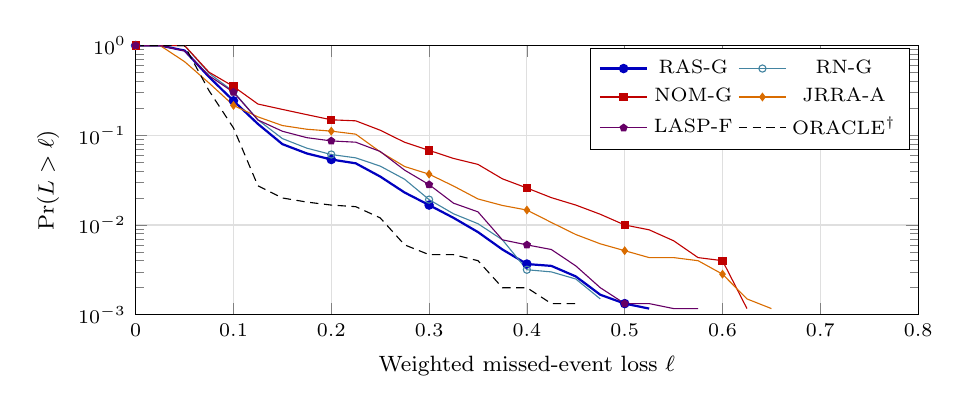
\begin{tikzpicture}
\begin{axis}[width=0.95\columnwidth,height=5.0cm,xlabel={Weighted missed-event loss $\ell$},ylabel={$\Pr(L>\ell)$},ymode=log,ymin=1e-3,ymax=1,xmin=0,xmax=0.8,grid=major,grid style={gray!25},tick label style={font=\scriptsize},label style={font=\footnotesize},legend style={font=\scriptsize,at={(0.99,0.99)},anchor=north east,legend columns=2},every axis plot/.append style={mark size=1.3pt,mark repeat=4}]

\addplot[blue!75!black,thick,mark=*] coordinates {(0.000,1.00000)(0.025,1.00000)(0.050,0.87967)(0.075,0.44650)(0.100,0.24217)(0.125,0.13367)(0.150,0.07967)(0.175,0.06267)(0.200,0.05367)(0.225,0.04867)(0.250,0.03467)(0.275,0.02300)(0.300,0.01667)(0.325,0.01200)(0.350,0.00833)(0.375,0.00533)(0.400,0.00367)(0.425,0.00350)(0.450,0.00267)(0.475,0.00167)(0.500,0.00133)(0.525,0.00117)};
\addlegendentry{RAS-G}
\addplot[cyan!60!black,mark=o] coordinates {(0.000,1.00000)(0.025,1.00000)(0.050,1.00000)(0.075,0.49167)(0.100,0.30667)(0.125,0.14850)(0.150,0.09183)(0.175,0.07183)(0.200,0.06100)(0.225,0.05600)(0.250,0.04533)(0.275,0.03233)(0.300,0.01917)(0.325,0.01333)(0.350,0.01033)(0.375,0.00683)(0.400,0.00317)(0.425,0.00300)(0.450,0.00250)(0.475,0.00150)};
\addlegendentry{RN-G}
\addplot[red!75!black,mark=square*] coordinates {(0.000,1.00000)(0.025,1.00000)(0.050,1.00000)(0.075,0.50450)(0.100,0.34983)(0.125,0.22283)(0.150,0.19417)(0.175,0.16967)(0.200,0.14867)(0.225,0.14483)(0.250,0.11383)(0.275,0.08350)(0.300,0.06783)(0.325,0.05517)(0.350,0.04733)(0.375,0.03267)(0.400,0.02583)(0.425,0.02017)(0.450,0.01667)(0.475,0.01317)(0.500,0.01000)(0.525,0.00883)(0.550,0.00667)(0.575,0.00433)(0.600,0.00400)(0.625,0.00117)};
\addlegendentry{NOM-G}
\addplot[orange!85!black,mark=diamond*] coordinates {(0.000,1.00000)(0.025,1.00000)(0.050,0.66133)(0.075,0.38250)(0.100,0.21500)(0.125,0.16033)(0.150,0.12833)(0.175,0.11667)(0.200,0.11117)(0.225,0.10283)(0.250,0.06533)(0.275,0.04483)(0.300,0.03683)(0.325,0.02717)(0.350,0.01950)(0.375,0.01650)(0.400,0.01467)(0.425,0.01067)(0.450,0.00783)(0.475,0.00617)(0.500,0.00517)(0.525,0.00433)(0.550,0.00433)(0.575,0.00400)(0.600,0.00283)(0.625,0.00150)(0.650,0.00117)};
\addlegendentry{JRRA-A}
\addplot[violet!80!black,mark=pentagon*] coordinates {(0.000,1.00000)(0.025,1.00000)(0.050,0.87233)(0.075,0.46133)(0.100,0.30183)(0.125,0.14800)(0.150,0.11083)(0.175,0.09400)(0.200,0.08650)(0.225,0.08367)(0.250,0.06600)(0.275,0.04083)(0.300,0.02817)(0.325,0.01750)(0.350,0.01400)(0.375,0.00683)(0.400,0.00600)(0.425,0.00533)(0.450,0.00350)(0.475,0.00200)(0.500,0.00133)(0.525,0.00133)(0.550,0.00117)(0.575,0.00117)};
\addlegendentry{LASP-F}
\addplot[black,densely dashed] coordinates {(0.000,1.00000)(0.025,1.00000)(0.050,0.99600)(0.075,0.31400)(0.100,0.12067)(0.125,0.02733)(0.150,0.02000)(0.175,0.01800)(0.200,0.01667)(0.225,0.01600)(0.250,0.01200)(0.275,0.00600)(0.300,0.00467)(0.325,0.00467)(0.350,0.00400)(0.375,0.00200)(0.400,0.00200)(0.425,0.00133)(0.450,0.00133)};
\addlegendentry{ORACLE$^\dagger$}
\end{axis}
\end{tikzpicture}

\caption{Complementary distribution of the loss at $\rho=1$.}
\label{fig:tail}
\end{figure}

\textbf{Risk budget and bandwidth.} Fig.~\ref{fig:pareto} illustrates the tradeoff between tail risk and provisioned bandwidth obtained by sweeping the multiplier $\lambda$. The CVaR decreased from 0.260 at $\lambda=0$ to 0.242 at $\lambda=8$, whereas the provisioned bandwidth increased from 40~Mb/s to 70~Mb/s. Notably, the setting $\lambda=0.5$ captured 80\% of this reduction with 52~Mb/s. Accordingly, a small multiplier captures most of the achievable tail reduction. Larger multipliers mainly add redundant streams whose value appears only in rare scenarios. In practice, an operator can select $\lambda$ at the knee of this frontier, and Proposition~\ref{prop:lag} gives each choice an approximate implicit CVaR budget. Every point of the frontier also dominates JRRA-A, which provisioned 141~Mb/s with a higher tail loss.

\begin{figure}[t]
\centering
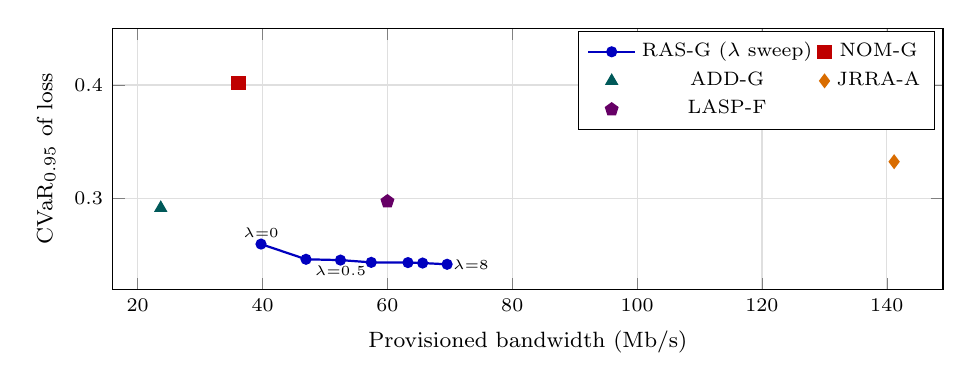
\begin{tikzpicture}
\begin{axis}[width=\columnwidth,height=4.9cm,xlabel={Provisioned bandwidth (Mb/s)},ylabel={CVaR$_{0.95}$ of loss},grid=major,grid style={gray!25},xmin=16,xmax=149,ymin=0.22,ymax=0.45,tick label style={font=\scriptsize},label style={font=\footnotesize},legend style={font=\scriptsize,at={(0.99,0.99)},anchor=north east,legend columns=2}]

\addplot[blue!75!black,thick,mark=*,mark size=1.6pt] coordinates {(39.75,0.2600)(46.96,0.2466)(52.48,0.2459)(57.41,0.2439)(63.29,0.2437)(65.64,0.2433)(69.56,0.2422)};
\addlegendentry{RAS-G ($\lambda$ sweep)}
\addplot[only marks,red!75!black,mark=square*,mark size=2.4pt] coordinates {(36.17,0.4016)};\addlegendentry{NOM-G}
\addplot[only marks,teal!70!black,mark=triangle*,mark size=2.4pt] coordinates {(23.69,0.2918)};\addlegendentry{ADD-G}
\addplot[only marks,orange!85!black,mark=diamond*,mark size=2.4pt] coordinates {(141.17,0.3325)};\addlegendentry{JRRA-A}
\addplot[only marks,violet!80!black,mark=pentagon*,mark size=2.4pt] coordinates {(60.00,0.2976)};\addlegendentry{LASP-F}
\node[font=\tiny,anchor=south,inner sep=2pt] at (axis cs:39.75,0.2600) {$\lambda{=}0$};
\node[font=\tiny,anchor=north,inner sep=2pt] at (axis cs:52.48,0.2459) {$\lambda{=}0.5$};
\node[font=\tiny,anchor=west,inner sep=2pt] at (axis cs:69.56,0.2422) {$\lambda{=}8$};
\end{axis}
\end{tikzpicture}

\caption{Tail loss versus provisioned bandwidth at $\rho=1$.}
\label{fig:pareto}
\end{figure}

\textbf{Load and disruption severity.} Fig.~\ref{fig:loadsev} illustrates the sensitivity of the compared methods to the load factor and to the disruption severity. RAS-G kept the lowest tail loss at every load factor and every severity level. The rate-centric baselines degraded fastest as the network became scarcer. When $\rho$ increased from 1 to 5, the tail loss of JRRA-A rose from 0.333 to 0.531 and that of LASP-F rose from 0.298 to 0.513. Over the same range, the tail loss of RAS-G rose only from 0.244 to 0.303. Similarly, the average recall of JRRA-A fell to 0.725 at $\rho=5$, whereas RAS-G retained 0.864. Under scarcity, the capacity shield left little room for redundant streams, and the margin over RN-G shrank to 0.005. The paired differences to RN-G were not significant at $\rho\in\{2,4\}$.

As the severity $\kappa_d$ increased from 0.5 to 2.5, the tail loss of RAS-G increased from 0.170 to 0.405. The tail loss of JRRA-A increased faster, from 0.209 to 0.624. RAS-G remained below RN-G at every severity, with Wilcoxon $p$-values of at most 0.041. However, for $\kappa_d\ge1.5$ the average recall of RAS-G fell below that of RN-G by up to 0.5 percentage points. This result exposes the tradeoff between average and tail performance under frequent disruptions.

\begin{figure*}[t]
\centering
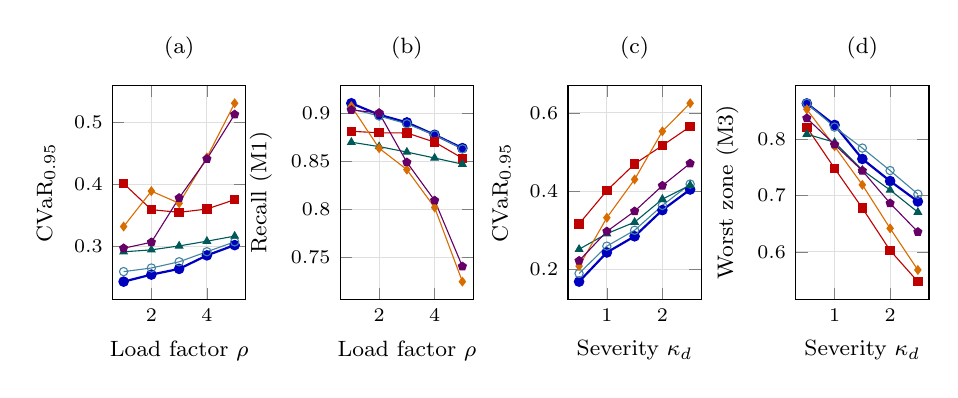
\begin{tikzpicture}
\begin{groupplot}[group style={group size=4 by 1,horizontal sep=1.2cm},width=0.27\textwidth,height=4.3cm,grid=major,grid style={gray!25},
 tick label style={font=\scriptsize},label style={font=\footnotesize},every axis plot/.append style={mark size=1.5pt},legend columns=6,legend style={font=\scriptsize,draw=none,column sep=6pt}]
\nextgroupplot[xlabel={Load factor $\rho$},ylabel={CVaR$_{0.95}$},title={\footnotesize (a)},legend to name=lsleg]
\addplot[blue!75!black,thick,mark=*] coordinates {(1.0,0.2439)(2.0,0.2552)(3.0,0.2644)(4.0,0.2861)(5.0,0.3026)};
\addlegendentry{RAS-G}
\addplot[cyan!60!black,mark=o] coordinates {(1.0,0.2600)(2.0,0.2658)(3.0,0.2758)(4.0,0.2920)(5.0,0.3079)};
\addlegendentry{RN-G}
\addplot[red!75!black,mark=square*] coordinates {(1.0,0.4016)(2.0,0.3596)(3.0,0.3553)(4.0,0.3606)(5.0,0.3757)};
\addlegendentry{NOM-G}
\addplot[teal!70!black,mark=triangle*] coordinates {(1.0,0.2918)(2.0,0.2950)(3.0,0.3013)(4.0,0.3089)(5.0,0.3171)};
\addlegendentry{ADD-G}
\addplot[orange!85!black,mark=diamond*] coordinates {(1.0,0.3325)(2.0,0.3894)(3.0,0.3699)(4.0,0.4436)(5.0,0.5307)};
\addlegendentry{JRRA-A}
\addplot[violet!80!black,mark=pentagon*] coordinates {(1.0,0.2976)(2.0,0.3072)(3.0,0.3785)(4.0,0.4412)(5.0,0.5127)};
\addlegendentry{LASP-F}
\nextgroupplot[xlabel={Load factor $\rho$},ylabel={Recall (M1)},title={\footnotesize (b)}]
\addplot[blue!75!black,thick,mark=*] coordinates {(1.0,0.9108)(2.0,0.8988)(3.0,0.8908)(4.0,0.8779)(5.0,0.8640)};
\addplot[cyan!60!black,mark=o] coordinates {(1.0,0.9049)(2.0,0.8975)(3.0,0.8894)(4.0,0.8777)(5.0,0.8632)};
\addplot[red!75!black,mark=square*] coordinates {(1.0,0.8816)(2.0,0.8800)(3.0,0.8798)(4.0,0.8703)(5.0,0.8535)};
\addplot[teal!70!black,mark=triangle*] coordinates {(1.0,0.8702)(2.0,0.8656)(3.0,0.8599)(4.0,0.8537)(5.0,0.8473)};
\addplot[orange!85!black,mark=diamond*] coordinates {(1.0,0.9077)(2.0,0.8639)(3.0,0.8416)(4.0,0.8021)(5.0,0.7248)};
\addplot[violet!80!black,mark=pentagon*] coordinates {(1.0,0.9038)(2.0,0.9007)(3.0,0.8492)(4.0,0.8094)(5.0,0.7407)};
\nextgroupplot[xlabel={Severity $\kappa_d$},ylabel={CVaR$_{0.95}$},title={\footnotesize (c)}]
\addplot[blue!75!black,thick,mark=*] coordinates {(0.5,0.1695)(1.0,0.2439)(1.5,0.2851)(2.0,0.3520)(2.5,0.4045)};
\addplot[cyan!60!black,mark=o] coordinates {(0.5,0.1903)(1.0,0.2600)(1.5,0.3005)(2.0,0.3639)(2.5,0.4184)};
\addplot[red!75!black,mark=square*] coordinates {(0.5,0.3168)(1.0,0.4016)(1.5,0.4698)(2.0,0.5166)(2.5,0.5649)};
\addplot[teal!70!black,mark=triangle*] coordinates {(0.5,0.2521)(1.0,0.2918)(1.5,0.3212)(2.0,0.3799)(2.5,0.4155)};
\addplot[orange!85!black,mark=diamond*] coordinates {(0.5,0.2089)(1.0,0.3325)(1.5,0.4302)(2.0,0.5529)(2.5,0.6245)};
\addplot[violet!80!black,mark=pentagon*] coordinates {(0.5,0.2228)(1.0,0.2976)(1.5,0.3490)(2.0,0.4143)(2.5,0.4711)};
\nextgroupplot[xlabel={Severity $\kappa_d$},ylabel={Worst zone (M3)},title={\footnotesize (d)}]
\addplot[blue!75!black,thick,mark=*] coordinates {(0.5,0.8645)(1.0,0.8261)(1.5,0.7655)(2.0,0.7261)(2.5,0.6897)};
\addplot[cyan!60!black,mark=o] coordinates {(0.5,0.8648)(1.0,0.8223)(1.5,0.7849)(2.0,0.7448)(2.5,0.7028)};
\addplot[red!75!black,mark=square*] coordinates {(0.5,0.8219)(1.0,0.7487)(1.5,0.6779)(2.0,0.6024)(2.5,0.5468)};
\addplot[teal!70!black,mark=triangle*] coordinates {(0.5,0.8097)(1.0,0.7952)(1.5,0.7456)(2.0,0.7101)(2.5,0.6707)};
\addplot[orange!85!black,mark=diamond*] coordinates {(0.5,0.8540)(1.0,0.7880)(1.5,0.7194)(2.0,0.6418)(2.5,0.5676)};
\addplot[violet!80!black,mark=pentagon*] coordinates {(0.5,0.8381)(1.0,0.7912)(1.5,0.7445)(2.0,0.6865)(2.5,0.6354)};
\end{groupplot}
\end{tikzpicture}
\\[1mm]\ref{lsleg}

\caption{Sensitivity to load (a, b) and disruption severity (c, d).}
\label{fig:loadsev}
\end{figure*}

\textbf{Ablation.} Table~\ref{tab:ablation} reports the change of each metric when one component of RAS-G is removed. The removal of route diversity caused the largest degradation, with a CVaR increase of 0.159. The nominal variant increased the tail loss by a similar amount (0.158), which confirms the value of scenario exposure. The capped additive surrogate reduced the average recall by 4.1 percentage points and increased the CVaR by 0.048. This result addresses RQ2 on overlapping camera views. The additive model overestimates the coverage of overlapping views and therefore stops adding streams too early. Restricting all cameras to the full mode increased the CVaR by 0.049 while consuming 65~Mb/s of additional bandwidth. The static survival ratio of the earlier controller design reached a similar tail loss ($+0.004$, $p=0.489$). However, the static ratio required 23~Mb/s of additional bandwidth because it overstates the damage on lightly loaded links. Finally, the ratio rule changed the results only marginally at the default load ($p=0.087$).

\begin{table}[t]
\caption{Ablation at $\rho=1$ (change relative to RAS-G)}
\label{tab:ablation}
\centering\footnotesize
\setlength{\tabcolsep}{4pt}
\begin{tabular}{@{}lcccc@{}}
\toprule
Variant & $\Delta$M1 & $\Delta$M2 & $\Delta$M3 & $\Delta$M4 (Mb/s)\\ \midrule
No CVaR term ($\lambda=0$) & $-0.006$ & $+0.016$$^{*}$ & $-0.004$ & $-17.7$ \\
Additive surrogate & $-0.041$ & $+0.048$$^{*}$ & $-0.031$ & $-33.7$ \\
Shortest route only & $-0.025$ & $+0.159$$^{*}$ & $-0.065$ & $-13.6$ \\
Full mode only & $+0.006$ & $+0.049$$^{*}$ & $-0.002$ & $+65.0$ \\
Nominal scenario only & $-0.029$ & $+0.158$$^{*}$ & $-0.077$ & $-21.2$ \\
Static survival ratio & $+0.004$ & $+0.004$ & $-0.002$ & $+22.9$ \\
Gain rule only & $+0.000$ & $+0.002$ & $+0.000$ & $+1.7$ \\
\bottomrule
\multicolumn{5}{@{}l}{\scriptsize $^{*}$Wilcoxon signed-rank $p<0.05$ for $\Delta$M2 over 15 topologies.}
\end{tabular}
\end{table}


\textbf{Robustness.} Fig.~\ref{fig:robust} illustrates three robustness tests at $\rho=1$. In Fig.~\ref{fig:robust}(a), the configurations were computed with $\kappa=0.87$ and evaluated under inter-view correlations between 0 and 0.8. RAS-G kept the lowest tail loss at every correlation level, and its CVaR rose from 0.198 to 0.321. From a correlation of 0.6, JRRA-A achieved a higher average recall than RAS-G (0.835 against 0.815 at 0.8). Therefore, a strongly correlated site requires a recalibrated $\kappa$.

In Fig.~\ref{fig:robust}(b), the controllers were trained at $\kappa_d=1$ and tested at higher severities. RAS-G remained well below JRRA-A and LASP-F at every tested severity. However, its advantage over RN-G was not significant at $\kappa_d\in\{1.5,2.0,2.5\}$ under the Wilcoxon test (0.368 against 0.367 at $\kappa_d=2$). Retraining on scenarios of the matched severity reduced the tail loss to 0.340 at $\kappa_d=2$ and to 0.415 at $\kappa_d=2.5$. Accordingly, the scenario generator must track the disruption statistics of the site.

In Fig.~\ref{fig:robust}(c), the number of training scenarios was varied from 25 to 500. The out-of-sample CVaR decreased from 0.312 to 0.241, which is consistent with the sample average approximation principle. Meanwhile, the decision time increased from 1.1~s to 2.4~s. The default of 300 scenarios therefore balances estimation quality against decision time.

\begin{figure*}[t]
\centering
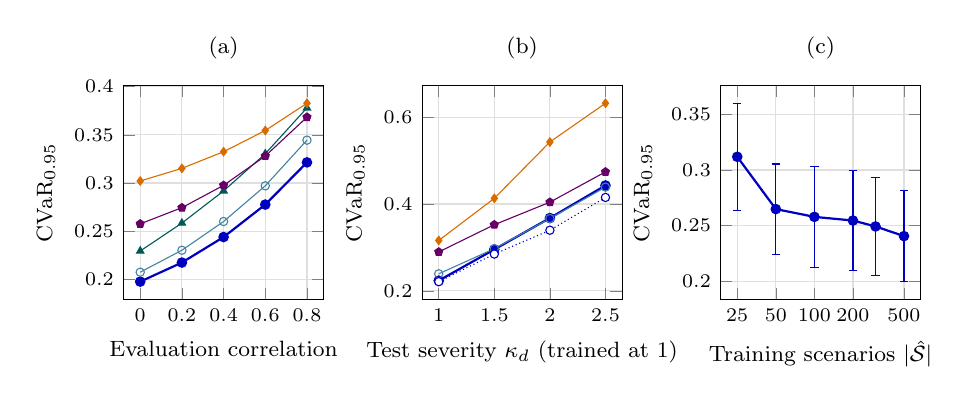
\begin{tikzpicture}
\begin{groupplot}[group style={group size=3 by 1,horizontal sep=1.25cm},width=0.34\textwidth,height=4.3cm,grid=major,grid style={gray!25},
 tick label style={font=\scriptsize},label style={font=\footnotesize},every axis plot/.append style={mark size=1.5pt},legend columns=7,legend style={font=\scriptsize,draw=none,column sep=6pt}]
\nextgroupplot[xlabel={Evaluation correlation},ylabel={CVaR$_{0.95}$},title={\footnotesize (a)},legend to name=robleg]
\addplot[blue!75!black,thick,mark=*] coordinates {(0.0,0.1976)(0.2,0.2174)(0.4,0.2439)(0.6,0.2776)(0.8,0.3214)};
\addlegendentry{RAS-G}
\addplot[cyan!60!black,mark=o] coordinates {(0.0,0.2074)(0.2,0.2302)(0.4,0.2600)(0.6,0.2971)(0.8,0.3445)};
\addlegendentry{RN-G}
\addplot[teal!70!black,mark=triangle*] coordinates {(0.0,0.2294)(0.2,0.2584)(0.4,0.2918)(0.6,0.3304)(0.8,0.3780)};
\addlegendentry{ADD-G}
\addplot[orange!85!black,mark=diamond*] coordinates {(0.0,0.3021)(0.2,0.3152)(0.4,0.3325)(0.6,0.3545)(0.8,0.3828)};
\addlegendentry{JRRA-A}
\addplot[violet!80!black,mark=pentagon*] coordinates {(0.0,0.2576)(0.2,0.2744)(0.4,0.2976)(0.6,0.3280)(0.8,0.3684)};
\addlegendentry{LASP-F}
\addlegendimage{blue!75!black,densely dotted,mark=*,mark options={solid,fill=white}}\addlegendentry{RAS-G (matched)}
\nextgroupplot[xlabel={Test severity $\kappa_d$ (trained at 1)},ylabel={CVaR$_{0.95}$},title={\footnotesize (b)}]
\addplot[blue!75!black,thick,mark=*] coordinates {(1.0,0.2236)(1.5,0.2955)(2.0,0.3677)(2.5,0.4428)};
\addplot[cyan!60!black,mark=o] coordinates {(1.0,0.2393)(1.5,0.2972)(2.0,0.3666)(2.5,0.4389)};
\addplot[orange!85!black,mark=diamond*] coordinates {(1.0,0.3161)(1.5,0.4131)(2.0,0.5429)(2.5,0.6321)};
\addplot[violet!80!black,mark=pentagon*] coordinates {(1.0,0.2897)(1.5,0.3524)(2.0,0.4043)(2.5,0.4741)};
\addplot[blue!75!black,densely dotted,mark=*,mark options={solid,fill=white}] coordinates {(1.0,0.2213)(1.5,0.2848)(2.0,0.3397)(2.5,0.4152)};
\nextgroupplot[xlabel={Training scenarios $|\hat{\mathcal S}|$},ylabel={CVaR$_{0.95}$},xmode=log,log basis x=10,title={\footnotesize (c)},xtick={25,50,100,200,500},xticklabels={25,50,100,200,500}]
\addplot[blue!75!black,thick,mark=*,error bars/.cd,y dir=both,y explicit] coordinates {(25,0.3119) +- (0,0.0481)(50,0.2649) +- (0,0.0405)(100,0.2579) +- (0,0.0451)(200,0.2546) +- (0,0.0446)(300,0.2493) +- (0,0.0440)(500,0.2406) +- (0,0.0409)};
\end{groupplot}
\end{tikzpicture}
\\[1mm]\ref{robleg}

\caption{Robustness to correlation mismatch (a), severity shift (b) and training size (c).}
\label{fig:robust}
\end{figure*}

\textbf{Literature-inspired profiles.} Under the RoundaboutHD-inspired profiles (8 topologies), RAS-G retained the lowest tail loss (CVaR$_{0.95}=0.276$), against 0.286 for RN-G, 0.309 for LASP-F and 0.387 for JRRA-A (28.6\% lower than JRRA-A). Provisioned bandwidth rose for all methods because the literature-inspired rates are higher, and the camera-side feature delay made the embedding mode less attractive on tight deadlines. These numbers remain a sensitivity study, not a claim of detector-calibrated accuracy.

\textbf{Larger networks.} The comparison was repeated on eight topologies with 48 cameras and 24 zones. RAS-G again achieved the lowest tail loss (0.087), against 0.097 for RN-G and 0.117 for JRRA-A. The denser camera coverage reduced the tail loss of all methods. In this setting, the difference to LASP-F (0.094) was not significant ($p=0.461$). However, LASP-F and JRRA-A provisioned 120~Mb/s and 276~Mb/s, whereas RAS-G provisioned 55~Mb/s. Additionally, both rate-centric baselines reached a higher average recall (0.948 and 0.949) than RAS-G (0.941).

\textbf{Optimality and scalability.} Table~\ref{tab:scale} compares RAS-G with the cut-based mixed-integer benchmark on small networks with 60 training scenarios. The benchmark is optimal for the tangent-cut approximation of~\eqref{eq:surrogate}, not for the original nonlinear program. The gap is expressed in loss units of the combined objective $\mathbb E[L]+\lambda\,\mathrm{CVaR}_{0.95}(L)$ and was evaluated with the exact (cut-based) recourse. HiGHS solved every benchmark instance to optimality of the approximated model. For the risk-neutral objective, the mean gap of RAS-G remained at or below 0.0022. For $\lambda=1$, the mean gap ranged from 0.0064 to 0.0174, whereas the static-survival design reached mean gaps of up to 0.0556. These results support RQ3 for the tested network sizes. On eight small instances, evaluating the nonlinear surrogate at the cut-based MILP solution increased mean loss by only 0.002 and CVaR$_{0.95}$ by 0.002 relative to the cut objective, consistent with Proposition~\ref{prop:cuts}.  The exact solve time for $\lambda=1$ grew from 9~s to 60~s as the network grew from 8 to 16 cameras. In contrast, RAS-G required 1.8~s for 24 cameras and 44~s for 96 cameras with 300 sampled scenarios in a single Python process. The frame-shedding linear program required below 12~ms per realized scenario in these measurements.

\begin{table}[t]
\caption{Optimality gap and runtime}
\label{tab:scale}
\centering\footnotesize
\setlength{\tabcolsep}{3.2pt}
\begin{tabular}{@{}rccccc@{}}
\toprule
Cameras & \multicolumn{2}{c}{Gap RAS-G} & Gap static & MILP (s) & RAS-G (s)\\
 & $\lambda=0$ & $\lambda=1$ & $\lambda=1$ & $\lambda=1$ & $\lambda=1$\\ \midrule
8 & 0.0022 & 0.0141 & 0.0556 & 9.2 & 0.16 \\
12 & 0.0014 & 0.0174 & 0.0449 & 26.2 & 0.34 \\
16 & 0.0004 & 0.0064 & 0.0196 & 59.5 & 0.54 \\
\midrule
24 & n/a & n/a & n/a & n/a & 1.81 \\
48 & n/a & n/a & n/a & n/a & 10.45 \\
72 & n/a & n/a & n/a & n/a & 22.58 \\
96 & n/a & n/a & n/a & n/a & 43.88 \\
\bottomrule
\multicolumn{6}{@{}l}{\scriptsize Mean absolute gaps in loss units over 5 topologies with 60 scenarios.}\\
\multicolumn{6}{@{}l}{\scriptsize Runtimes above 16 cameras use 300 scenarios and 3 topologies.}
\end{tabular}
\end{table}


\section{Discussion and Limitations}
The results answer the three research questions with measured caveats. For RQ1, the CVaR term reduced the tail loss at the default setting and at every tested severity. However, the reduction was not significant at load factors of 2 and 4 or under an unmodeled severity shift. Scenario-based semantic orchestration produced the larger part of the gain. For RQ2, the calibrated surrogate improved the average recall, the tail loss and the worst-zone coverage relative to the capped additive surrogate. For RQ3, the controller stayed close to the exact optimum for the risk-neutral objective. The gap was larger for the risk-aware objective, which motivates stronger search moves in future designs.

Several limitations must be considered when interpreting these findings. First, the default mode profiles and visibility factors are synthetic. A literature-inspired RoundaboutHD profile set~\cite{lin2025easemcvt} is reported as a sensitivity check, including camera-side feature-extraction delay, but it is not a detector calibration on WILDTRACK~\cite{chavdarova2018wildtrack}. A YOLO-based multi-view measurement campaign is required before deployment claims can be made. Second, the flow-level simulator does not capture packet-level queueing, transport dynamics or radio scheduling. Third, the calibration factor $\kappa$ depends on the inter-view correlation, and Fig.~\ref{fig:robust}(a) shows that a strongly correlated site needs recalibration. Fourth, the benefit of the CVaR term depends on a scenario generator that matches the disruption statistics of the site. Fifth, suppressed feeds were modeled as random events rather than adaptive attacks. Finally, the results separate network and service resilience from the robustness of the detector to image manipulation.

From a practical perspective, the proposed controller requires only telemetry that edge orchestrators already collect. With 300 training scenarios in a single Python process, RAS-G decided in about 1.9~s for 24 cameras and about 44~s for 96 cameras; the per-scenario frame-shedding LP stayed below 12~ms. These runtimes support closed-loop reconfiguration on the order of tens of seconds to a few minutes, which matches slow wireless/edge capacity drift and planned maintenance windows rather than sub-frame radio scheduling. The role of 6G in this work is therefore architectural: native AI service placement, semantic traffic classes and multi-access edge capacity that make joint mode--route--server decisions meaningful. The numerical study uses 5G-Advanced/6G-like flow-level capacities, not a packet-level 6G air-interface model. For 96 cameras, the independent search runs of each stage can be executed in parallel to shorten the decision time. Moreover, every RAS-G configuration satisfied the nominal capacity shield in all evaluated topologies. The bandwidth provisioned by RAS-G also remained well below that of the rate-centric JRRA-A configuration. The controller's risk term should be read as a tunable penalty, not as a hard CVaR certificate for arbitrary out-of-sample disruptions.

\section{Conclusion}
This paper presented RAS-6G, a risk-aware semantic utility orchestration framework for multi-camera surveillance in 6G-oriented edge networks. The framework jointly selects camera modes, routes and edge servers under a CVaR-oriented objective on severity-weighted missed-event loss, with a hard CVaR constraint in the offline model and a Lagrangian penalty in the online controller. A correlation-calibrated surrogate accounts for overlapping views, and a greedy controller with a load-aware recourse approximation supports online operation. In the evaluated scenarios, the proposed controller reduced the tail loss by 26.6\% relative to adapted JRRA while provisioning 59\% less bandwidth. At the default setting, the explicit CVaR term added a 6.2\% tail reduction relative to the risk-neutral variant. The proposed framework has emerged as a promising basis for resilient and task-oriented video service management at the wireless edge. As part of our future work, we plan to investigate measured detector profiles on real multi-view datasets and packet-level 5G-Advanced emulation. We also plan to investigate fast intra-interval reconfiguration, which could close part of the remaining gap to the clairvoyant benchmark.


\section*{Acknowledgments}
The authors received no external funding for this work.

\section*{Data and Code Availability}
The simulator, experiment scripts, raw JSON results and figure/table generators are provided as supplementary material and in the public repository \url{https://github.com/papersC/RiskAware-Semantic-Surveillance}. All random streams are seeded for reproduction.

\section*{Generative AI and AI-Assisted Technologies}
Generative AI tools were used for drafting and editing assistance. All technical content, algorithms, experimental design, results and conclusions were verified by the authors, who take full responsibility for the manuscript.

\bibliographystyle{IEEEtran}
\bibliography{references}
\end{document}
